\subsection{Simulation results} 
The backstepping controller was also tested on the a trajectory tracking task akin to the one seen in Section \ref{sec:fbl_sim}. The reference trajectory is expressed in \ref{eq:pos_ref} and \ref{eq:yaw_ref}, with the same parameters $r = \qty{5}{\meter}$, $d = 5$ and $k = 10$. 
\\With the current controller, which is far more robust than of the previous one, we can also afford to start from an initial condition corresponding to a nonzero initial tracking error, i.e., the origin.

The comparison between the reference and the actual trajectory of Ingenuity is shown in Figure \ref{fig:BS_trajectory}. Notice that the robot is able to follow the desired path with a good approximation, while recovering both the initial position error and the final one (generated by the abrupt change in the reference). 
\begin{figure}[H]
    \centering
    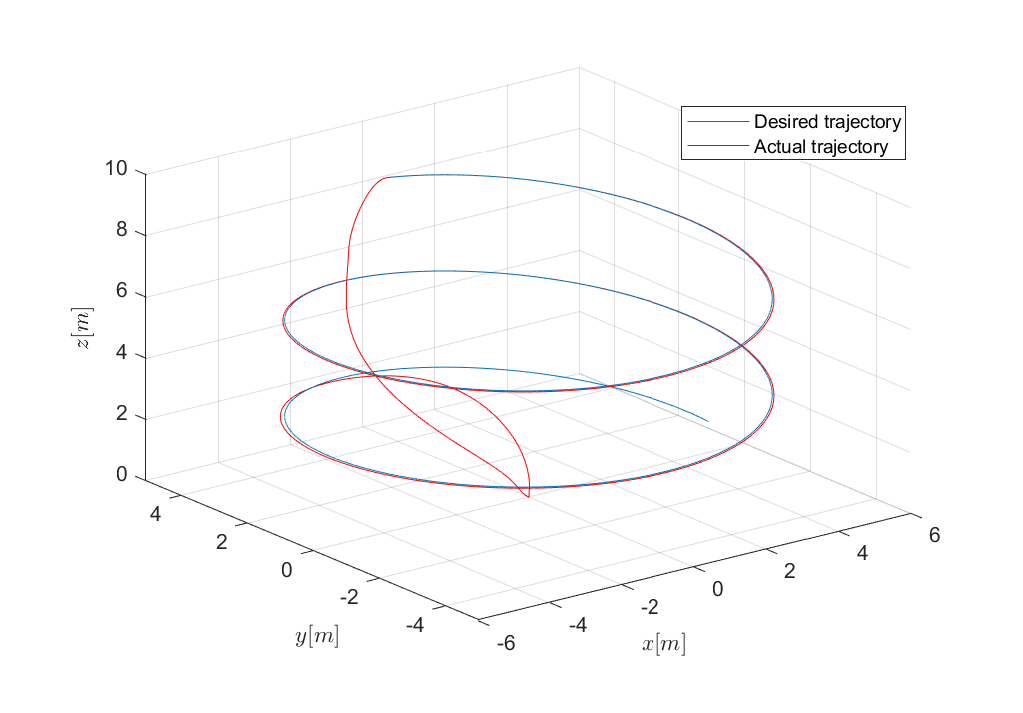
\includegraphics[scale=0.5]{figures/BS_trajectory}
    \caption{Trajectory tracking.}
    \label{fig:BS_trajectory}
\end{figure}
As theoretically expected, the controller exploits the roll and pitch dynamics to impart the desired behavior to the remainder of the system (see Figure \ref{fig:BS_attitude}). 
\begin{figure}[H]
    \centering
    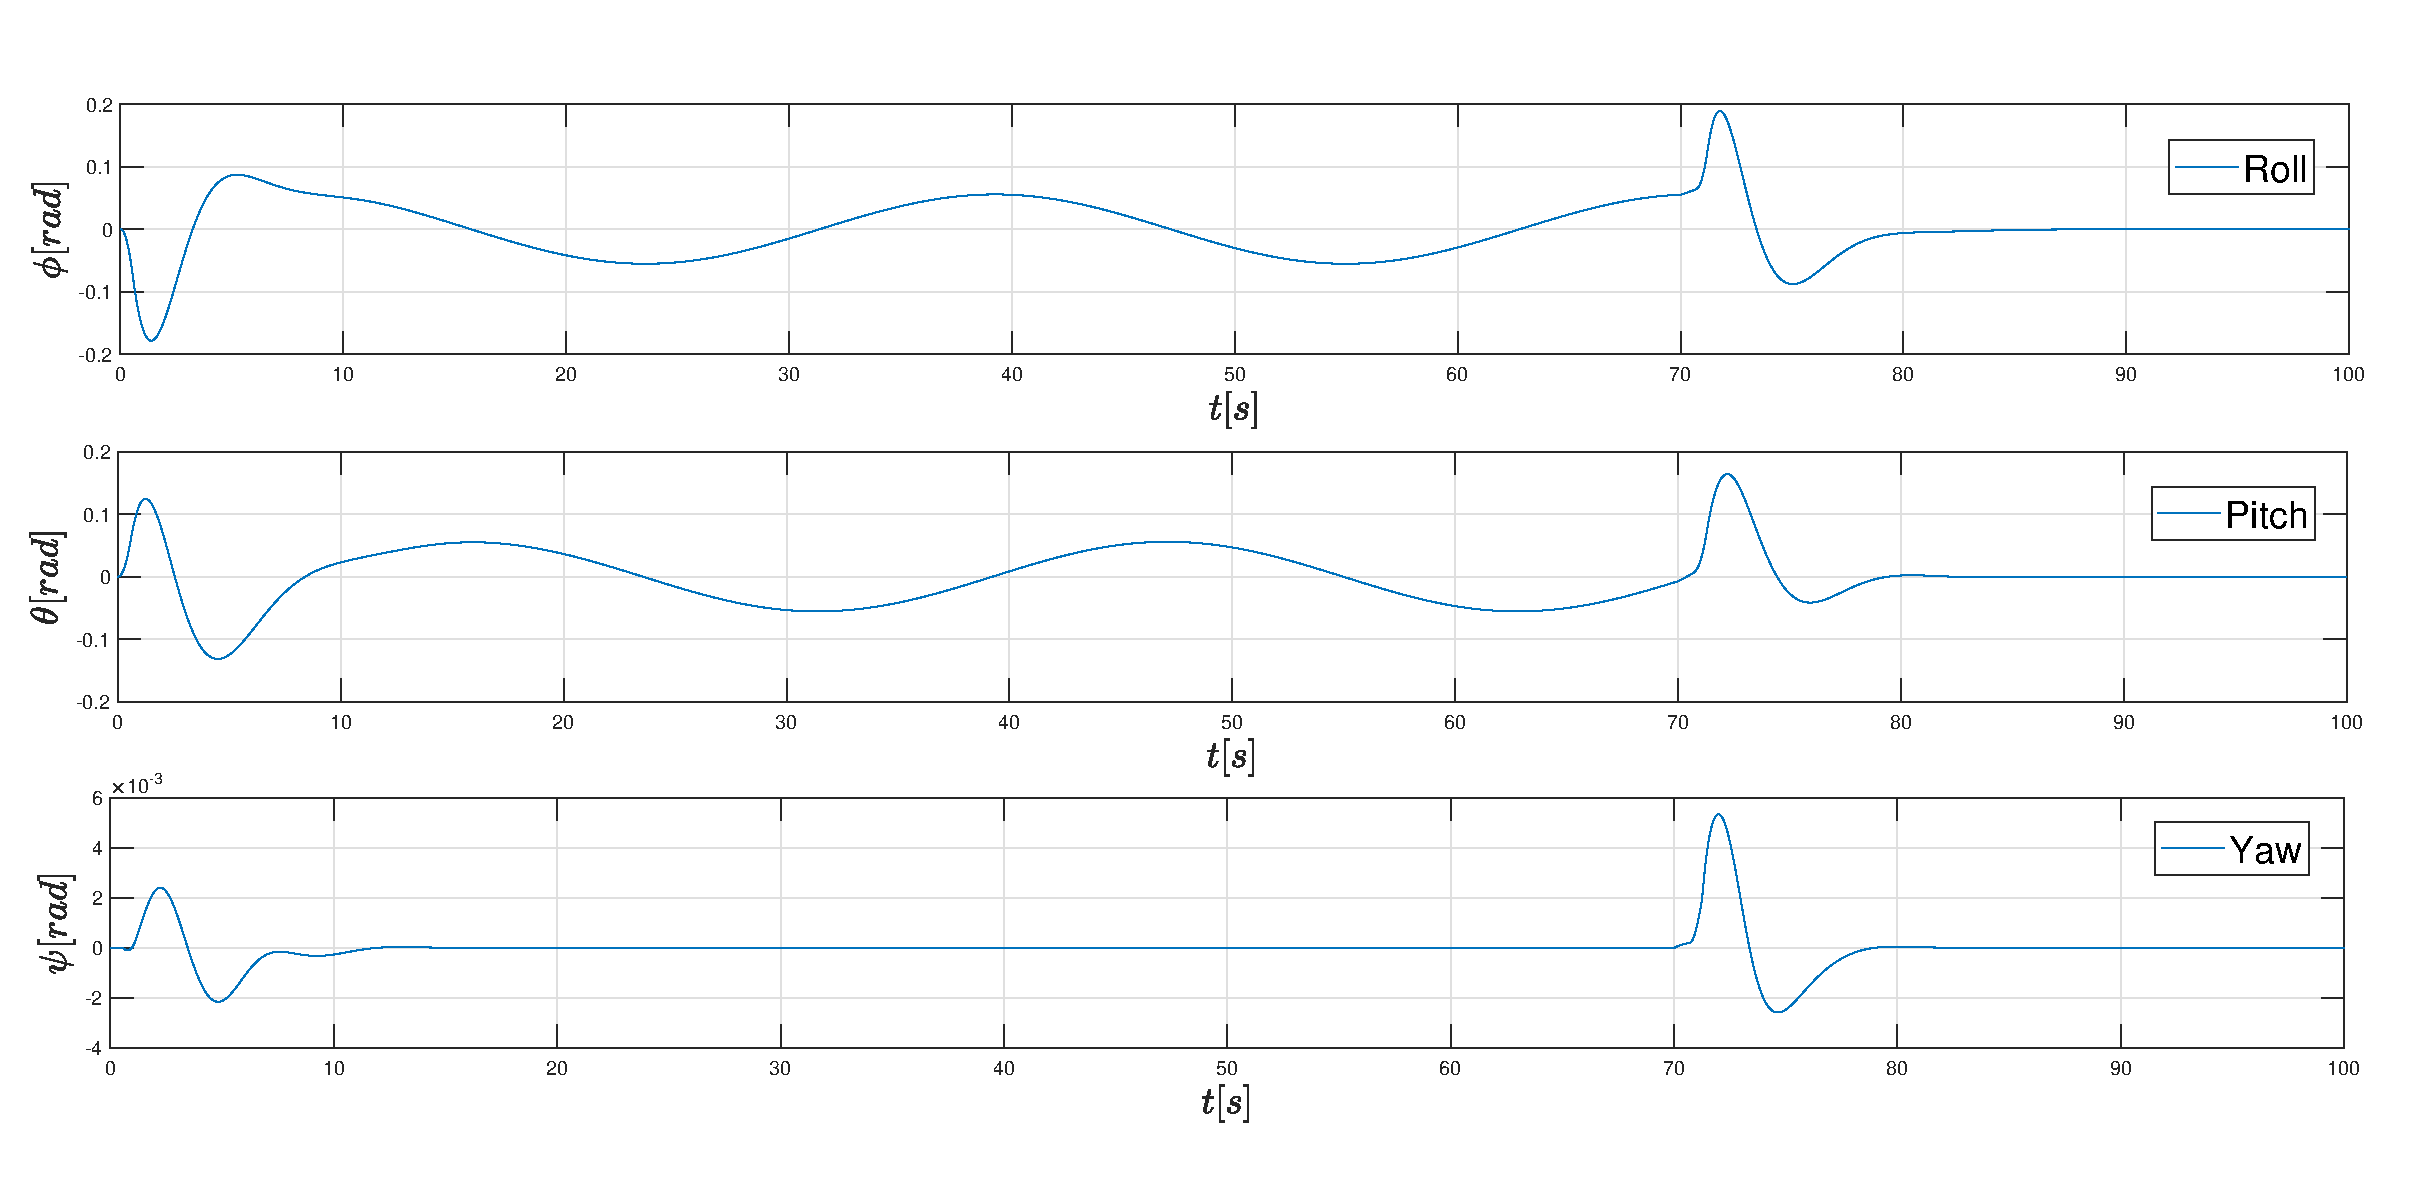
\includegraphics[scale=0.2]{figures/BS_attitude}
    \caption{Evolution of the roll, pitch and yaw angles respectively.}
    \label{fig:BS_attitude}
\end{figure}
Finally, the necessary control inputs, adequately saturated according to the constraints \ref{eq:omega_u_constraint} - \ref{eq:beta_constraint} so as to reflect the actual physical limitations of the actuators, are depicted in Figures \ref{fig:BS_angles} and \ref{fig:BS_omega}. 
\\ We can therefore state that the controller is not only robust to external disturbances, but also to these types of constraints.
\begin{figure}[H]
    \centering
    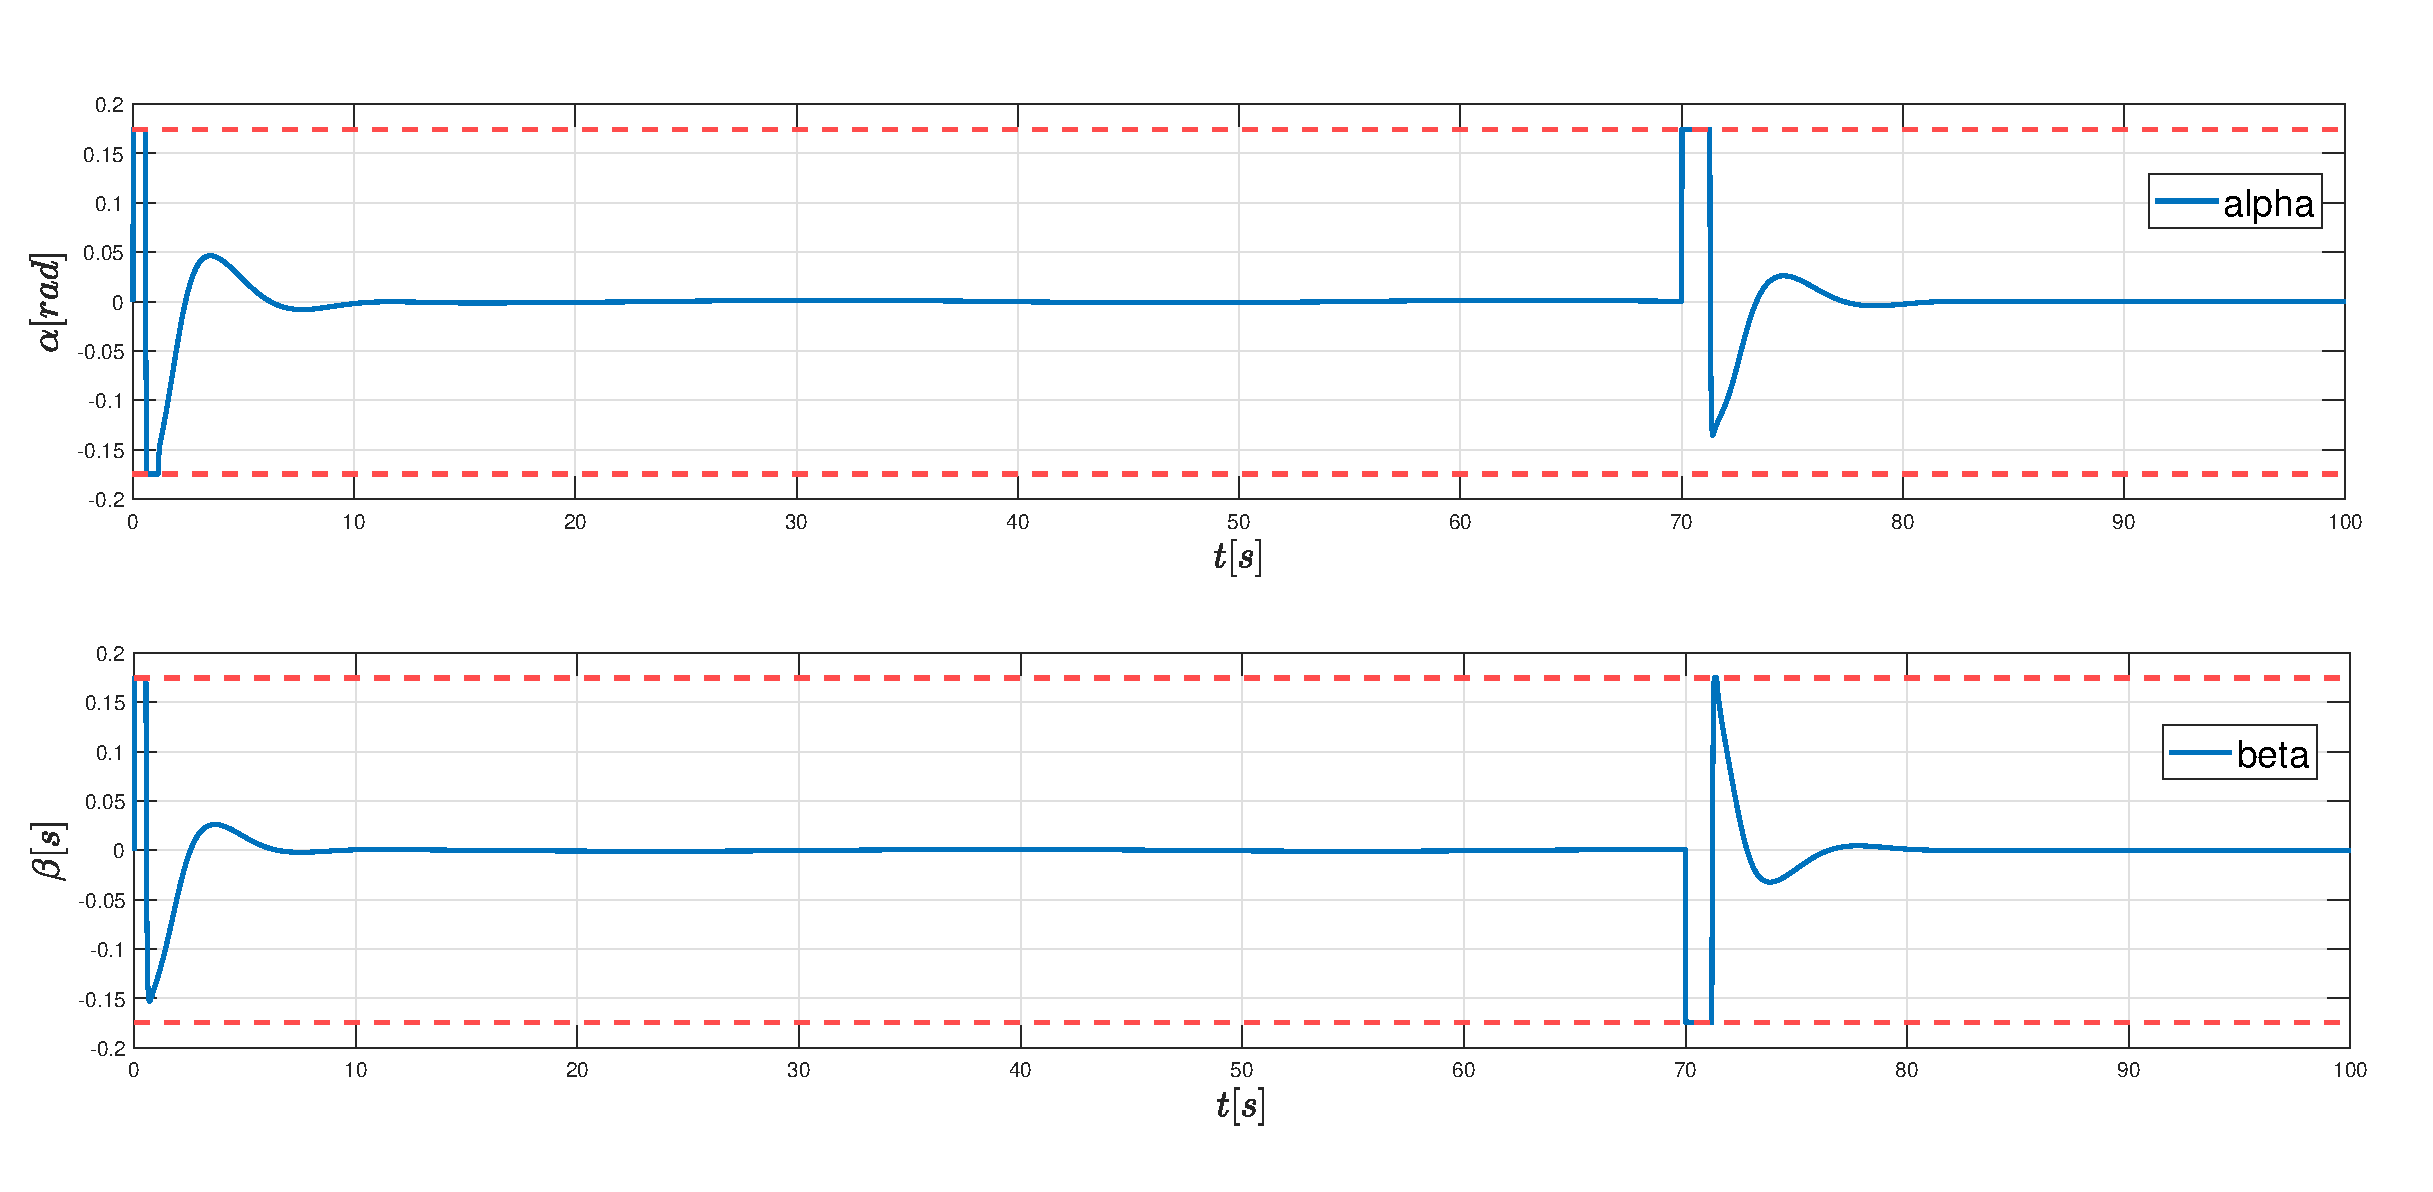
\includegraphics[scale=0.2]{figures/BS_angles}
    \caption{Angles $\alpha$ and $\beta$ of the swashplate.}
    \label{fig:BS_angles}
\end{figure}
\begin{figure}[H]
    \centering
    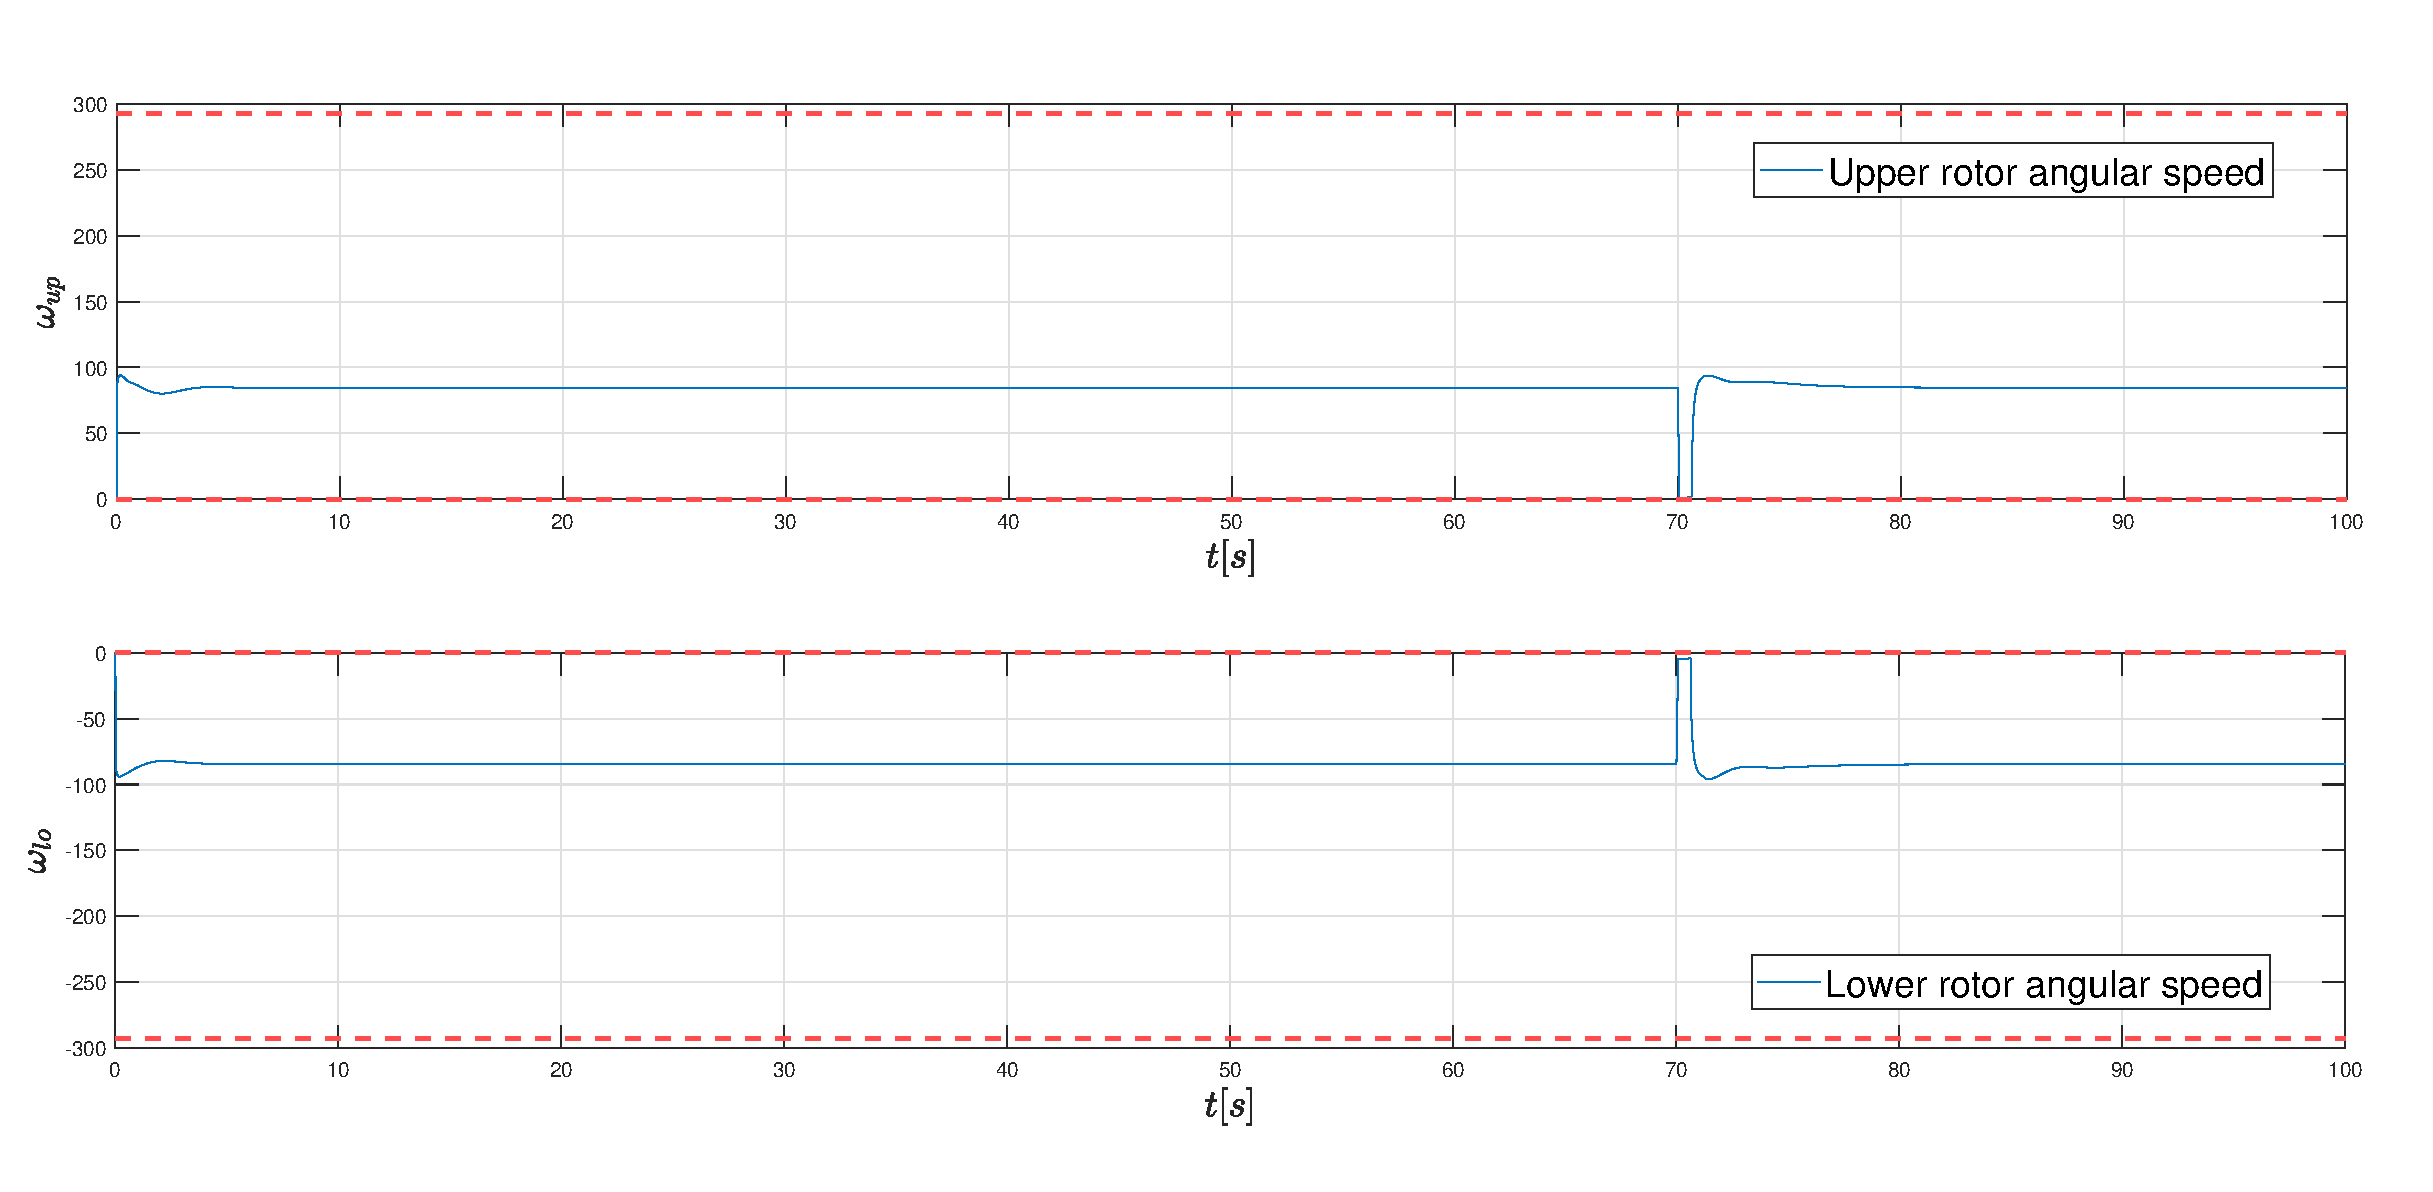
\includegraphics[scale=0.2]{figures/BS_omega}
    \caption{Angular velocities of the upper and lower rotor respectively.}
    \label{fig:BS_omega}
\end{figure}

